\chapter{Related Work}
\label{ch:related_work}
Many approaches have been proposed aiming for deploying DNN on mobile device, either in algorithm or hardward aspect. In this chapter, we will discuss more about the main optimization scheme we choose, which is quantisation, and then existing DNN accelerators hardware design.
\section{Quantization}
Quantization maps data to a smaller set of quantization levels. The principle is to minimize the error between the reconstructed data from the quantized one and the original data. The quantization level essentially reflects the bits required to represent the data. Reduced data bits comes with several benefits including reduced storage costs, memory transactions and computational cost. There are ways to quantization, from simplest uniform distance between each quantization \figref{quant_types}(a) level to special mapping function such as \textit{log} function so that distance between quantization steps are of logarithm relation \figref{quant_types}(b); and even more advanced approaches like clustering data into groups with k-means, requiring look up table for the mapping and computation \figref{quant_types}(c). The simplest quantization also known as \textit{linear quantization} related closely to this project, and we're going to focus on it particularly.
\begin{figure}
    \centering
    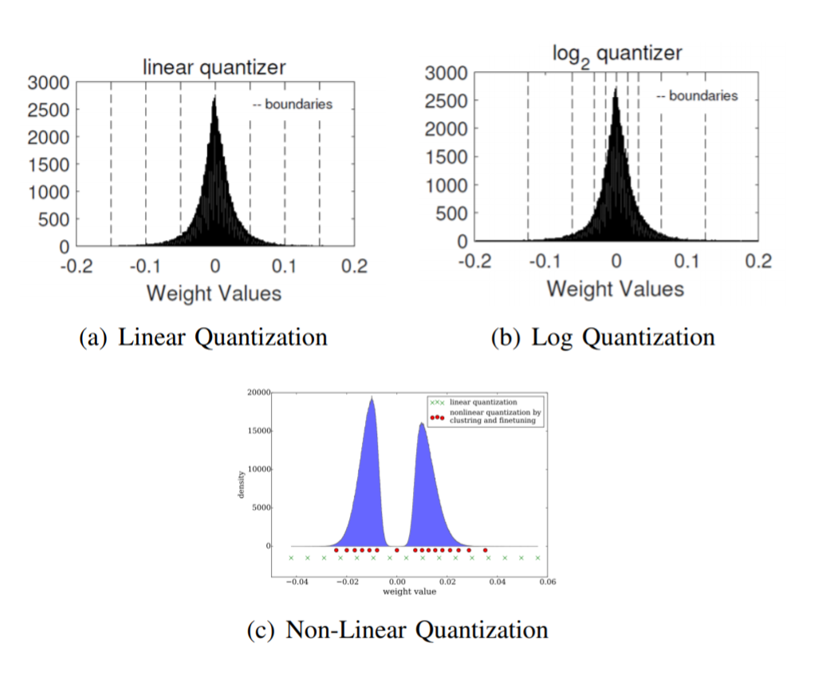
\includegraphics[width=0.8\linewidth]{inc/2_related_work/figure/quantization_types.png}
    \caption{Various methods of quantization; taken from \cite{lognet}\cite{DeepCompression}}
    \label{fig:quant_types}
\end{figure}
\subsection{fixed point quantisation}
More related to this work, researches find the numerical requirement for even the latest DNN model inference stage far from the commonly used 32/64 bit floating-point format. \cite{FixedPoint} quantize the models to fixed point with ${L_2}$ error minimization, achieved \textbf{0.89\%} MCR (miss classification rate) on \textbf{MNIST} with 5 bits weights in comparison to \textbf{0.81\%} MCR with floating point weights.
\subsection{ternary to binary quantisation}
Some researchers have tried extreme quantization down to 2bits ternary weights such as in TWNs\cite{Ternary} and even binary weights in BinaryNet \cite{BinaryNet}, to binarize both weight and activation as in XNOR-net\cite{XnorNet}. \\
TWNs minimizes the Euclidian distance between the full precision weights $\boldsymbol{W}$ and ternary-valued weights $\boldsymbol{W^t}$ along with a non-negative scaling factor $\alpha$ in \eqref{eq:twn} achieving \textbf{99.35\%}, \textbf{92.56\%}, \textbf{84.2\%} on \textbf{MNIST}, \textbf{CIFAR-10}, \textbf{ImageNet(top-5)} dataset respectively.  
\begin{equation}
\begin{aligned}\label{eq:twn}
    \alpha^*, \boldsymbol{W^{t*}} = \mathop{\arg\min}_{\alpha,\boldsymbol{W^t}} = \|\boldsymbol{W}-\alpha\boldsymbol{W^t}\|^2_2 \\  
\text{s.t }\alpha\geq0,\boldsymbol{W^t_i}\in\{1,0,-1\}, i=1,2,...,n.
\end{aligned}
\end{equation}
BinaryNet constrains both weights and activations to either +1 or -1 with 
\begin{equation}
    \begin{aligned}\label{eq:bn}
        x^b=\text{Sign}(x)=\begin{cases}
                        +1 &\text{if \(x\geq0\)}, \\
                        -1 &\text{otherwise},
                    \end{cases}
    \end{aligned}
\end{equation}
achieving \textbf{0.96\%} , \textbf{10.15\%} error rate on \textbf{MNIST} , \textbf{CIFAR-10} dataset respectively.
And finally the Xnor-net put their emphasis on the scaling factor $\alpha^*$ and $\boldsymbol{K}$ between layers that first computes the floating point value of an output tensor, then take the sign of it for the binarized activation for the input of next layer.
\begin{equation}
    \begin{aligned}\label{eq:xnornet}
        \alpha^*=\frac{\boldsymbol{W^T}\text{sign ($\boldsymbol{W}$)}}{n}=\frac{\Sigma\|\boldsymbol{W_i}\|}{n}=\frac{1}{n}\|\boldsymbol{W}\|_{l1} \\
        \boldsymbol{K}=\frac{\Sigma\|\boldsymbol{I}_{:,:,i}\|}{c} * \frac{1}{w \times h}
    \end{aligned}
\end{equation}
In a Xnor-net particularly the convolutional operation seen in \figref{xnor_operation} can be appriximated by:
\begin{equation}
    \begin{aligned}\label{eq:xnorop}
        \boldsymbol{I}*\boldsymbol{W}\approx(sign(\boldsymbol{I}) * sign(\boldsymbol{W}))\odot\boldsymbol{K}\alpha
    \end{aligned}
\end{equation}
where $\boldsymbol{I}$, $\boldsymbol{W}$ denotes the input, weight tensors of a layer. Additionally, they discovered that regular batch-normalization layer position between convolution and activation function is unfriendly to binarization algorithm, by moving convolution layer after the activation function instead further boost the accuracy, achieving \textbf{69.2\%} top-5 accuracy on \textbf{ImageNet} using \textbf{AlexNet} model. By adopting binarization scheme, XNOR and bitcount operations can be applied to save computational cost at inference stage, with ~\textbf{58x} reported speed up against CPU time. \\
Pushing the limit to binarization hurts the accuracy by a large margin, worth mentioning that in Xnor-net they didn't quantize the first and the last layer of the convolution, which bear too much information to be discarded.
\begin{figure}
    \centering
    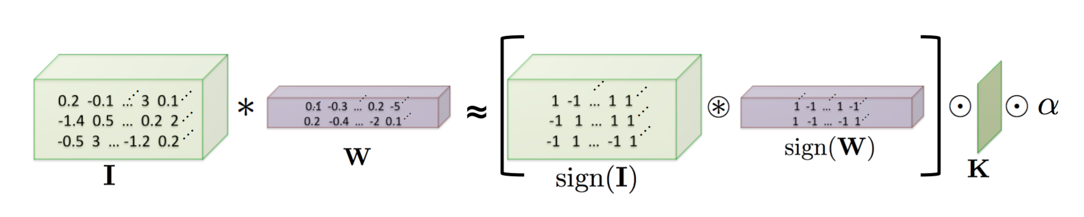
\includegraphics[width=0.8\linewidth]{inc/2_related_work/figure/xnor_operation.png}
    \caption{Convolution with XNOR-Bitcount in XNOR-net; taken from \cite{XnorNet}}
    \label{fig:xnor_operation}
\end{figure}
 
\subsection{8-bit quantization on modern models}
More practically, modern deep models have been showed to work on 8 bits quantization on both weights and activations \cite{TensorRT8bit}. Taking advantage of Nvidia's bulit-in INT8 operations on their GPUs, they developed a CUDA library in TensorRT with an algorithm minimizing loss of information when quantizing trained model without further fine tuning or retraining. Starting with the tensor approximation with quantized tensor:
\begin{equation}
    \begin{aligned}\label{eq:tensorrtop}
    \textbf{Tensor Values}\approx\textbf{FP32 scaling factor}*\textbf{INT8 array}
    \end{aligned}
\end{equation}
 The scaling factor determines the mapping of the quantized level to the original value, for example a scaling factor of $\frac{127}{2.7}$ maps the original data 2.7 to  quantized data 127. This is always a trade-off process between range and precision: the larger the scaling is, the larger the range, and the smaller the precision. The scaling process also includes the clipping of data exceeding a pre-defined threshold as seen in \figref{tensorrt_thresold}, and the threshold is in fact the scaling factor times the maximum level of the quantization, which is 127 in INT8 case.
\begin{figure}
    \centering
    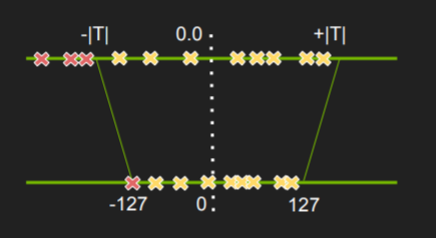
\includegraphics[width=0.5\linewidth]{inc/2_related_work/figure/tensorrt_thresold.png}
    \caption{Information loss is minimized through careful choice of saturation threshold; taken from \cite{TensorRT8bit}}
    \label{fig:tensorrt_thresold}
\end{figure}
\\
Therefore the main challenge here is the choice of the scaling factor.As stated in the work, INT8 model encodes the same information as the original FP32 model, the choosing of the scaling factor is a process of minimizing the loss of information, which can be measured by Kullback-Leibler divergence as the relative entropy or information divergence \eqref{eq:kl_div} between two discrete probability distributions $\boldsymbol{P}$, $\boldsymbol{Q}$. They propose a \textbf{Calibration Dataset} to be run on FP32 format inference, collecting histograms of activations, and then pick threshold that minimize the KL divergence by generating many quantized data distributions with different saturation thresholds. This process is said to take only a few minutes on a desktop workstation. \\ 
\begin{equation}
    \begin{aligned}\label{eq:kl_div}
    \textbf{KL\_Divergence} ( \boldsymbol{P} , \boldsymbol{Q} ) := \textbf{SUM} ( \boldsymbol{P[i]} * log ( \frac{ \boldsymbol{P[i]}}{\boldsymbol{Q[i]}} ) , i)
    \end{aligned}
\end{equation}
The resulting INT8 model achieves no more than \textbf{0.46\%} extra error rate if even not lesser, at the same time speeding up from \textbf{1.62x} to \textbf{3.67x} depending on the inference batch size ( from 1 to 128) on their processor DRIVE PX2, dGPU. \\
In \autoref{ch:low prec NN} we propose a similar yet simpler scheme to search for the desirable quantization thresholds; although our approach involves no calibration after the training, it requires re-training on low-precision inference, and is likely to be slower than train-then-fine-tune scheme in this work. However, we believe that re-training on ultra-low-precision model ( $<$ 8 bits) is still necessary.

\section{Hardware design}
Recently researches related to deep neural network accelerator are blooming rapidly. They typically start off with a core algorithm simplifying the NN model, then combining either micro-architectural optimization such as low-precision arithmetic units or system level optimization involving data compression between the chip and the off-chip memory, delicate buffer design, sparsity-aware zero-skipping operations and so on. \\
We are going to focus on several works that inspire us the most, including modified classic systolic-array style processor operating on a granularity of rows, SIMD (single instruction multiple data) style processor coupled with re-configurable arithmetic unit being able to operate on 1-16 bits respectively.
From these works, we conclude that slashing down memory access counts either from on-chip or off-chip is of upmost importance for chip power efficiency, through further low-bit operation optimization the memory transaction frequency can be furthered improved. 
\subsection{Dataflow optimization: row stationary}
Eyeriss\cite{Eyeriss} analyzes existing accelerator work in a now widely used manner, classifying them into \textit{Weight Stationary}, \textit{Output Stationary}, \textit{No Local Reuse} three dataflows that reuse data differently, and propose a novel processing dataflow coined \textit{Row Stationary} as in \figref{row_stationary}. \\
\begin{figure}
    \centering
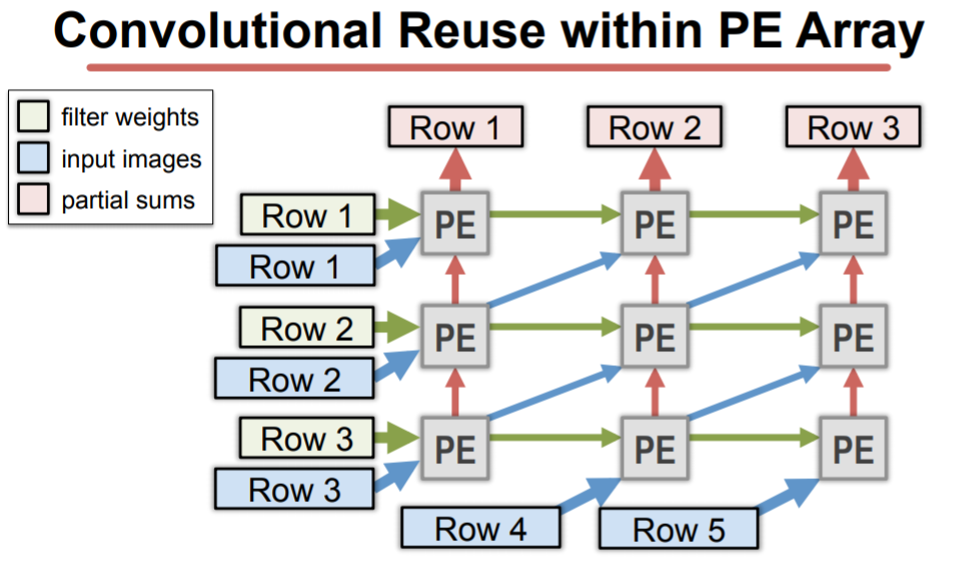
\includegraphics[width=0.6\linewidth]{inc/2_related_work/figure/row_stationary.png}
    \caption{Row stationary: rows passed to processing elements as unit; taken from \cite{EyerissSlide}}
    \label{fig:row_stationary}
\end{figure}
The dataflow finely captures all sources of data reuse opportunities ranging from convolution reuse, batching, filter reuse. The work also adopts various optimization methods such as zero-gated register file, running-length coded data in-and-out of the chip, dynamic voltage and frequency scaling and so on. The work consisting of 168 PE with 16-bit fixed-point multipliers tapes out to have a peak performance of \textbf{42 GMACS}, operating avergely on \textbf{278mW}.

\subsection{Sub-word parallelism arithmetic unit}
\cite{PrecisionScalableVLSI} is one of the pioneering re-configurable low-precision processor for DNN. The 16-bit multiplier in each PE can be re-configured into one 1-16 bit multiplier, the resulting switching activity and critical path then scale with the configuration, allowing possible lower power supply at constant frequency according to power estimation equation $\boldsymbol{\alpha CfV^2}$ as in \figref{pre_scal_envi} (a), the unused logics are gated accordingly to prevent unwanted power dissipation. In terms of dataflow, the weights are shared along a PE row, the inputs are shared along a PE column in contrast; worth noting that a large shifting FIFO for input data is implemented so it propagates input data to adjacent PE column, this also indicates that the PE adopts \textit{output stationary} scheme. The work has a peak performance of \textbf{102 GOPS}, operating on \textbf{76mW} ( AlexNet ) and a maximum of \textbf{2.6TOPS/W} power efficiency. \\
\begin{figure}[t]
    \centering
    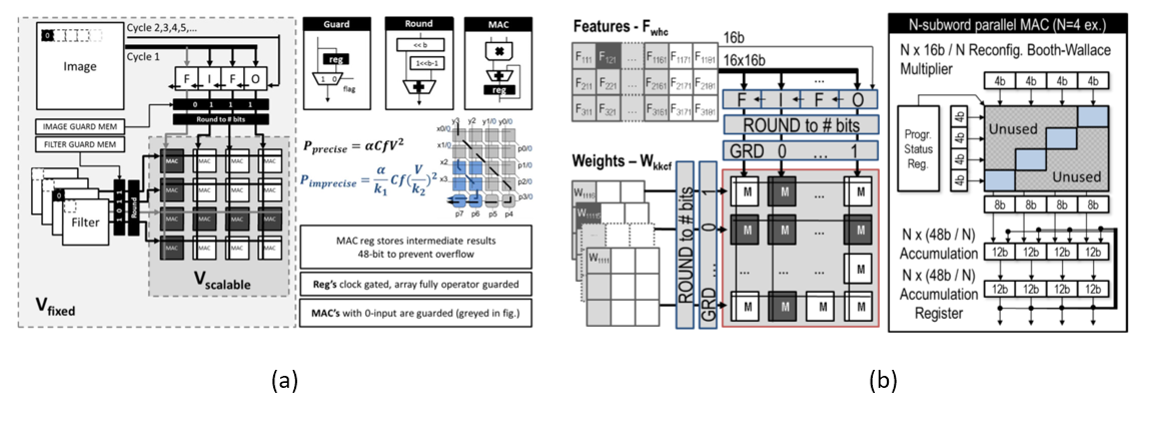
\includegraphics[width=1\linewidth]{inc/2_related_work/figure/precision_scalable_envision.png}
    \caption{(a) Precision re-configurable multiplier and (b)Sub-word parallelism re-configurable multiplier; taken from \cite{PrecisionScalableVLSI}\cite{ENVISION} }
    \label{fig:pre_scal_envi}
\end{figure}
\cite{ENVISION} inherits from \cite{PrecisionScalableVLSI}. Instead of a multiplier operating on 1 pair of variable bit-length data, this work proposes multiplier with $\boldsymbol{N}$=1,2,4 sub-word parallelism, in other words, a maximum of $\boldsymbol{N}$x peak performance as in \figref{pre_scal_envi} (b). The work has a peak performance \textbf{102N*GOPs}, operating from \textbf{7.5-300mW} and a maximum of \textbf{10TOPS/W} power efficiency. \\

By \textit{output stationary} scheme indicates both works above captures less convolutional reuse, and having sub-word parallelism means large local output register which renders row stationary dataflow inapplicable.
\begin{figure}[t]
    \centering
    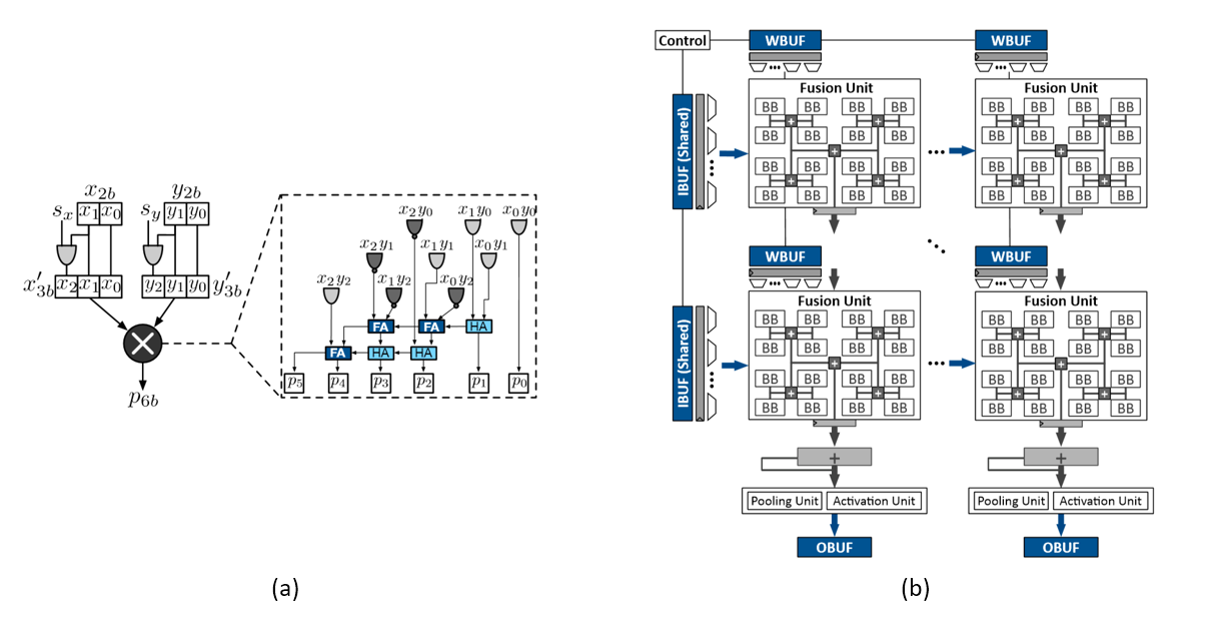
\includegraphics[width=0.7\linewidth]{inc/2_related_work/figure/bit_fusion.png}
    \caption{(a)BitBricks computing ternary multiply and add (b)Systolic-array processing architecture; taken from \cite{BitFusion}}
    \label{fig:bit_fusion}
\end{figure}
\subsection{Bit-level re-configurable arithmetic unit}

\cite{BitFusion} bears the most similarity to our work. A atomic processing block \textit{BitBricks} is proposed, which is effectively a ternary (-1,0,+1) mutliply and add unit with a 6b output as in \autoref{fig:bit_fusion} (a). 16 \textit{BitBricks} are put together inside one \textit{Fusion Unit}, offering 1,2,4,8,and 16 fused-BitBricks with varying operand bitwidths, output bitwidth and level of parallelism. The \textit{Fusion Units} are arranged in systolic-array manner, propagating partial sum vertically to output register and buffer as in \autoref{fig:bit_fusion} (b). The synthesized result are used to conducted extensive experiments comparing against other works. They claim to offer \textbf{3.9x} speed up and \textbf{5.1x} energy saving over \cite{Eyeriss} under same area, frequency and process technology; also they claim to match the performance of 250W Titan Xp using INT8 vector instructions, while consuming only \textbf{896mW}. \\
To have the best flexibility as this work does, an 6b output 2b multiplier would be inefficient area-wise to some degree, also considering a 16 \textit{BitBrick} fused 16-bit multiplier is essentially a 16 6-bit multiplier-adder tree, possibly introducing large area overhead in comparison to a modern 16-bit booth algorithm multiplier.
 \\

Works from above provide us several great starting points, involving \textit{row stationary} dataflow, re-configurable low-precision multiplier-add unit, SIMD architecture design. 
\iffalse
\begin{itemize}
    \item \textcolor{purple}{How does related work "relate" to your research question?}
    \item \textcolor{purple}{Does it provide a starting point?}
    \item \textcolor{purple}{Does it provide evidence that you are posing a good research question?}
    \item \textcolor{purple}{Does it provide a different approach to a similar research hypothesis that you can compare to?}
\end{itemize}
\fi